\chapter{Architettura iniziale}
\label{cha:architettura_iniziale}

In questo capitolo viene descritto lo stato iniziale di SATAYO, la sua complessità
e i problemi di scalabilità che hanno portato alla necessità di ripensare l'architettura
del progetto.

\section{Struttura del progetto}
\label{sec:struttura}

Il progetto SATAYO è strutturato in modo tale da permettere la distribuzione del
lavoro su più macchine virtuali. In questo modo, dal punto di vista teorico, dovrebbe
essere più semplice scalare l'applicazione in base alla quantità e alla dimensione
dei domini che vengono analizzati dalla piattaforma.

\begin{figure}[h!]
  \centering
  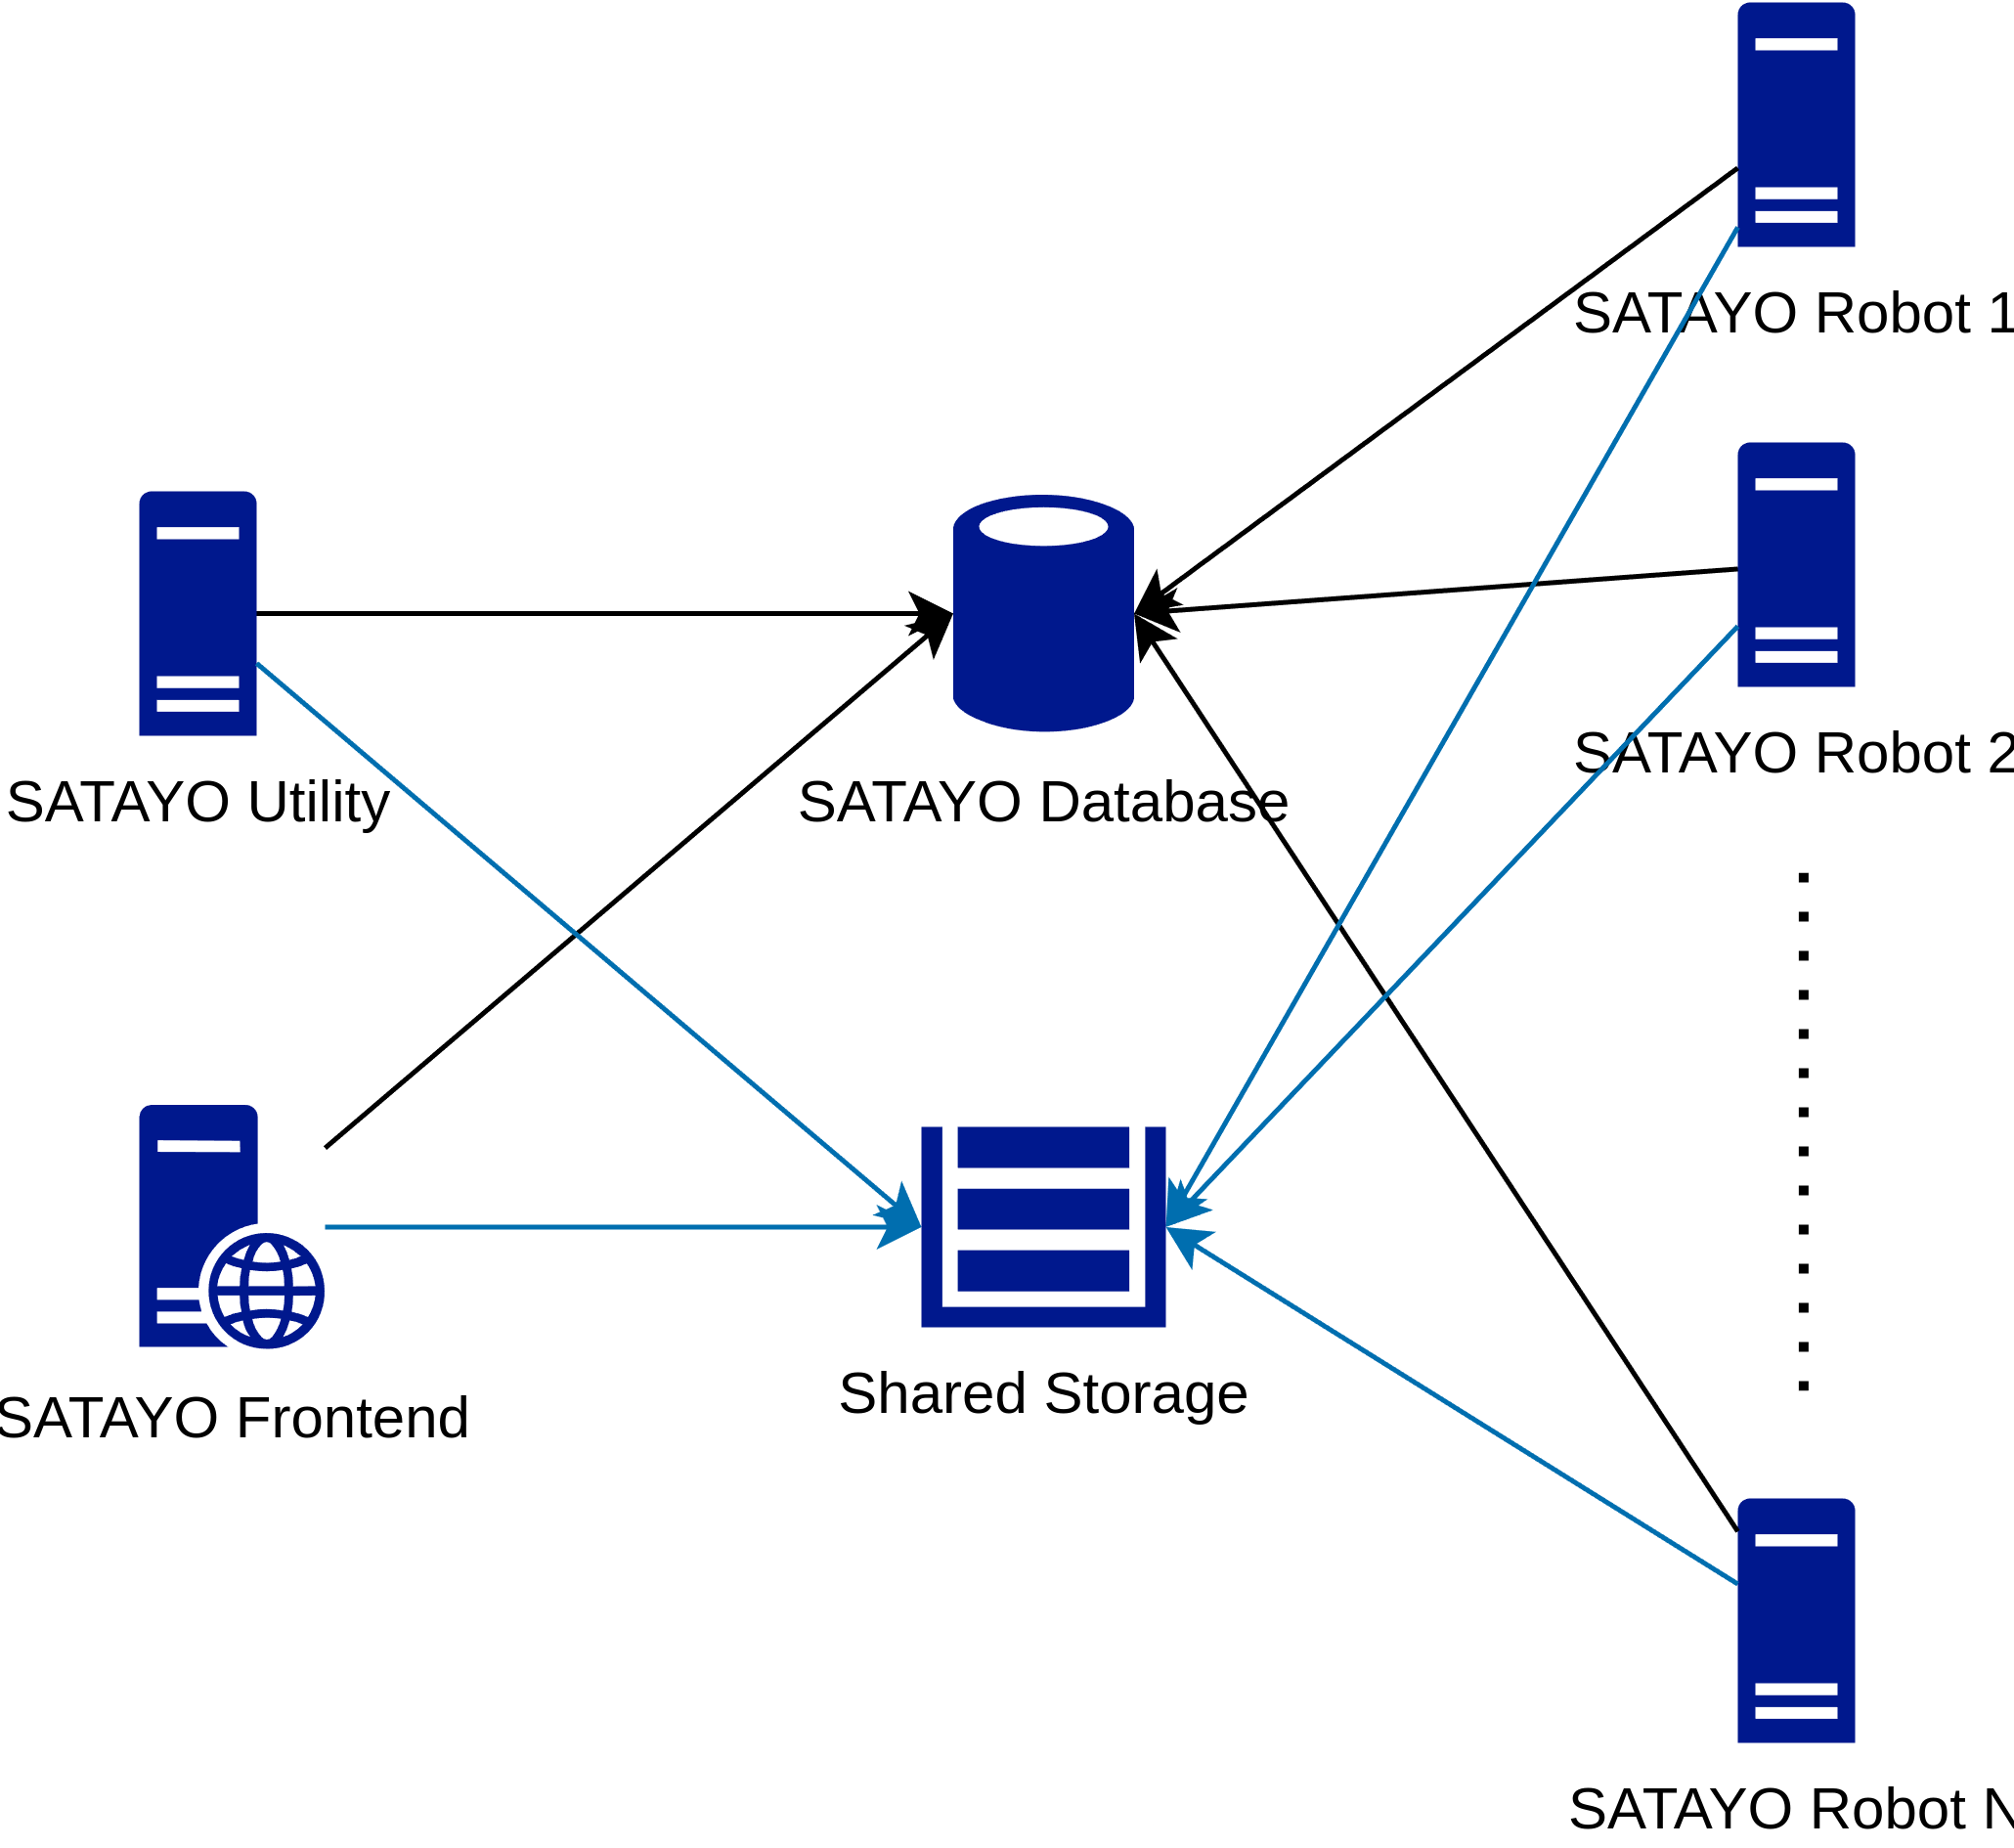
\includegraphics[width=.6\linewidth]{images/SATAYO_infrastructure_old.png}
  \caption{Vecchia infrastruttura di SATAYO}
  \label{fig:infra_old}
\end{figure}

Come si nota in figura \ref{fig:infra_old}, sono presenti tre categorie di macchine
con compiti distinti:

\begin{itemize}
  \item \textbf{SATAYO Frontend:} dedicata all'hosting del webserver con cui
    clienti e analisti si interfacciano per utilizzare la piattaforma. Questa macchina
    ha la necessità di interfacciarsi con il database, per leggere i dati
    generati da SATAYO e per inserire nuovi domini o informazioni relative a
    questi nella piattaforma. La stessa macchina ha inoltre bisogno di permessi di
    lettura sullo storage condiviso, in cui vengono salvate le evidenze trovate
    sulle varie piattaforme OSINT da SATAYO, per presentarle agli analisti che ne
    devono valutare la correttezza e gravità;

  \item \textbf{SATAYO Utility:} la sua funzione principale è quella di eseguire
    fasi molto scalabili orizzontalmente; fasi cioè, il cui tempo di esecuzione
    e carico sul sistema non dipende affatto o dipende in minima parte dal
    numero di input. Esempi specifici di queste esecuzioni possono essere lo scraping
    di siti web o di canali Telegram. Come la SATAYO Frontend anche SATAYO
    Utility comunica con il database, principalmente per inserire dati, e con lo
    storage condiviso per salvare evidenze collezionate da fonti varie;

  \item \textbf{SATAYO Robot:} argomento principale di questo elaborato, ha il compito
    di eseguire tutte le fasi legate ad un particolare dominio. Generalmente si
    tratta di programmi e tool open-source o di terze parti che lavorano su
    input singoli, non permettendo così una parallelizzazione analoga alle fasi Utility.
    Altra particolare caratteristica delle macchine Robot, che verrà analizzata più
    nel dettaglio al punto \ref{sub:robots}, è la necessità di eseguire le
    operazioni secondo un insieme di dipendenze. Per esempio, una funzione che
    ritorna una lista di servizi online a cui sono iscritti i dipendenti tramite
    email aziendali, deve essere eseguita dopo la fase che si occupa di raccogliere
    la lista di dipendenti di una determinata azienda. Questa famiglia di
    macchine, come la SATAYO Utility, si interfaccia direttamente con il
    database e con lo storage condiviso.
\end{itemize}

In fine è presente il database, il quale è ospitato su una macchina dedicata per
poter garantire una performance migliore. Quest'ultima, analogamente allo storage
condiviso, è protetta da policy di sicurezza più strette rispetto alle altre
macchine che hanno bisogno di comunicare e interagire con la rete esterna.

\subsection{Macchine Robot}
\label{sub:robots}

Di seguito verranno trattati più approfonditamente l'architettura, il
funzionamento e il controllo delle macchine Robot.

Come visto in precedenza queste macchine eseguono operazioni secondo un grafo di
dipendenze, le quali sono definite in modo implicito nei metadati delle singole fasi.
Con il termine \textit{dipendenze implicite} si intende che non è presente una rappresentazione
in cui si può osservare chiaramente l'ordine con cui devono essere eseguite le fasi,
ma bensì sono presenti delle impostazioni che definiscono, per ogni funzione, la
famiglia di fasi che si devono essere concluse prima che possa essere eseguita
quest'ultima.

L'esecuzione delle fasi viene gestita in modo piuttosto rudimentale: su ogni istanza
Robot è presente uno script Python \texttt{satayo.py} il quale viene eseguito da
un Crontab secondo un intervallo regolare di 5 minuti. Questo script è a tutti gli
effetti il controllore locale della macchina Robot, ha il compito di eseguire le
fasi presenti nella coda di quell'istanza e di controllare lo stato di
esecuzione di esse. Più nel dettaglio lo script esegue le seguenti operazioni:

\begin{itemize}
  \item controlla se l'esecuzione avviata con il cronjob precedente è ancora attiva,
    in tale caso non viene avviata nessuna nuova fase. In caso l'esecuzione precedente
    sia terminata si controlla che non ci siano stati errori nell'esecuzione, in
    caso positivo viene salvato sul database l'errore e gli eventuali messaggi
    di log.

  \item è selezionata la prossima fase da eseguire tramite lookup sulla tabella di
    coda nel database. Si eseguono dei controlli per verificare che le
    dipendenze di quest'ultima siano soddisfatte. Infine si avvia l'esecuzione effettiva
    della task.

  \item una volta terminata l'esecuzione vengono salvati i risultati dell'operazione,
    gli eventuali messaggi di log, lo stato finale dell'esecuzione, e la
    macchina rimane in attesa del prossimo cronjob.
\end{itemize}

Si possono immediatamente notare delle forti inefficienze, le quali saranno trattate
dettagliatamente al punto \ref{sec:problemi}:

\begin{itemize}
  \item l'intervallo del Crontab è stato calcolato in modo arbitrario secondo una
    stima della media pesata dei tempi di esecuzione delle varie fasi. Ciò
    significa che alcune esecuzioni sono molto più rapide rispetto all'intervallo
    e viene quindi sprecato tempo macchina;

  \item su ogni istanza può essere eseguita soltanto una fase alla volta, non è
    supportata l'esecuzione parallela sulla stessa macchina. La scelta fatta per
    cercare di mitigare questo problema è stata duplicare l'istanza su più macchine
    indipendenti e implementare la logica per gestire la distribuzione della coda.
\end{itemize}

L'approccio descritto è il risultato di un'aggiunta incrementale di funzionalità,
effettuata mantenendo la semplice struttura iniziale, ormai inadatta al carico
di lavoro e alla complessità del progetto.

La coda di esecuzione e i metadati delle fasi verranno trattati al punto
\ref{sec:database} assieme ad altri dettagli relativi al database.

\section{Struttura database}
\label{sec:database}

Il database di SATAYO, inizialmente formato da circa 50 tabelle, ne conta ad oggi
oltre 130. Non essendo possibile citare e descriverle tutte, vengono riportate
quelle principali e più inerenti ai problemi e alle modifiche che verranno
descritte al capitolo \ref{cha:nuova_architettura}.

\textbf{\textit{INSERIRE ER TABELLE (2 cluster): ui\_org, domain, research | tool\_progress,
tool, host, log}}

\subsection{Gestione clienti, domini e ricerche}
\label{sub:db:mgmt}

Il primo cluster di tabelle, rappresentato sulla sinistra in figura \textbf{\textit{X}}
forma il cuore del database di SATAYO, queste sono infatti tabelle che
contengono i dati del cliente, dei domini da analizzare e delle ricerche OSINT effettuate
sui vari domini. Nel dettaglio le tabelle rappresentate contengono le seguenti
informazioni:

\begin{itemize}
  \item \textbf{ui\_org:} contiene le informazioni relative ai clienti, quali:
    date di inizio e fine del contratto, collegamenti a software ERP interno,
    tipologia di contratto e funzionalità abilitate e altre informazioni di
    natura burocratica. Nel contesto tecnico svolge la funzione di permettere una
    gestione d'insieme dei domini e delle ricerche di un determinato cliente;

  \item \textbf{domain:} racchiude i domini monitorati per un determinato
    cliente. Oltre al dominio stesso contiene anche altre informazioni di contesto
    quali: keyword per eseguire ricerche online, nomi degli account di piattaforme
    di social media per verificare le informazioni esposte pubblicamente e formato
    delle mail aziendali per enumerare i dipendenti.

  \item \textbf{research:} in fase di progettazione iniziale, è stato individuato
    come requisito la possibilità di offrire uno storico della propria esposizione
    in rete al cliente. Ciò ha portato alla necessità di implementare questa
    tabella che ha il compito di rendere discrete le ricerche che vengono
    effettuate, permettendo quindi una visualizzazione distinta nel tempo dell'andamento
    delle evidenze ed esportabile in un report.
\end{itemize}

\subsection{Gestione fasi}
\label{sub:db:tasks}

Il secondo cluster, presente sulla destra della figura \textbf{\textit{X}}
contiene invece informazioni di natura operativa, quali code di esecuzione e metadati
delle fasi. Le funzionalità principali sono le seguenti:

\begin{itemize}
  \item \textbf{tool:} è una lista statica dei tool OSINT implementati su SATAYO,
    che ad oggi sono oltre 60. Contiene il nome dei singoli tool, l'ordine in
    cui devono essere eseguiti, assieme a metadati usati per la distribuzione su
    più host e per la gestione da frontend;

  \item \textbf{host:} un'altra lista statica contenente tutti gli hostname, e altre
    informazioni di gestione, delle macchine che formano la piattaforma SATAYO, come
    visto in figura \ref{fig:infra_old}. Al momento sono presenti 12 macchine
    Robot. Le informazioni contenute in questa tabella hanno la funzione principale
    di gestire la distribuzione delle fasi tra le diverse macchine Robot;

  \item \textbf{tool\_progress:} contiene lo stato di esecuzione delle singole
    fasi. Più nel dettaglio contiene informazioni quali: lo stato, cioè se una task
    può essere eseguita, è in esecuzione o è terminata con errore o con successo,
    e l'orario di inizio e di fine dell'esecuzione. Inoltre contiene anche le
    seguenti informazioni: tool da eseguire, host su cui viene eseguito e
    ricerca su cui caricare le evidenze collezionate dal tool;

  \item \textbf{log:} semplice tabella utilizzata per salvare messaggi di log
    provenienti dalle esecuzioni dei vari tool. Contiene il tempo di creazione del
    log, la gravità e il messaggio di log stesso. È utile per individuare problemi
    durante le esecuzioni di task direttamente dal frontend.
\end{itemize}

\pagebreak
\section{Problemi con architettura corrente}
\label{sec:problemi}

In seguito ad un'analisi di carico e ad una proiezione del numero di domini da
monitorare nei prossimi mesi, sono risultati immediatamente evidenti i problemi di
scalabilità che si sarebbero presentati se si fosse mantenuta l'architettura attuale.

Come accennato nelle sezioni precedenti, l'implementazione corrente permette di
scalare orizzontalmente in modo teoricamente semplice: se c'è bisogno di ulteriore
tempo di esecuzione è sufficiente aggiungere un'altra macchina Robot,
configurarla secondo una data documentazione e aggiungere eventuali entry nel
database. Questa può essere una valida soluzione in caso non sia necessario eseguire
la procedura molto spesso. Contrariamente, se fosse necessario scalare in modo più
che lineare, questa soluzione porterebbe ad un \textbf{notevole dispendio di
tempo} per la configurazione iniziale, ma soprattutto per la gestione e
manutenzione futura del sistema.

Un altro problema, a cui porterebbe un simile approccio, è lo \textbf{spreco di
risorse}: dal momento che l'implementazione attuale non può sfruttare al meglio
multipli core, per utilizzare in modo efficiente le risorse messe a disposizione
dall'infrastruttura sottostante, è necessario creare macchine con requisiti
minimi. Prendendo come riferimento la guida di Ubuntu Server\footnote{\url{https://ubuntu.com/server/docs/system-requirements}},
sistema operativo utilizzato su tutte le istanze, e aumentando lievemente le
risorse minime per poter eseguire anche le fasi più computazionalmente intensive,
si ottengono dei requisiti di 2 CPU core, 8GB di RAM e 60GB di spazio di
archiviazione. Questo porta il totale di risorse in utilizzo, considerando solo
le macchine Robot, a 24 CPU core, 96GB di RAM e 720GB di spazio di archiviazione,
la maggior parte delle quali non è possibile sfruttare appieno.

Terza criticità è la gestione dei log, i quali al momento vengono collezionati
tramite query direttamente sul database di SATAYO. Questo può portare ad alcune situazioni
in cui certi errori non vengono riportati correttamente; un esempio può essere
il caso in cui si perda la connessione con il database, la fase andrebbe in errore
ma non verrebbe correttamente riportato il messaggio di log.